% do not change these two lines (this is a hard requirement
% there is one exception: you might replace oneside by twoside in case you deliver 
% the printed version in the accordant format
\documentclass[11pt,titlepage,oneside,openany]{article}
\usepackage{times}


\usepackage{graphicx}
\usepackage{subcaption}
\usepackage{latexsym}
\usepackage{amsmath}
\usepackage{amssymb}
\usepackage{hyperref}

% Tables
\usepackage{pgfplots, pgfplotstable}
\usepgfplotslibrary{colorbrewer}
\pgfplotsset{compat=1.13}
\pgfplotsset{cycle list/Set1-6}
\usepackage{booktabs}
\usepackage{multirow}

\usepackage{ntheorem}

% \usepackage{paralist}
\usepackage{tabularx}

% this packaes are useful for nice algorithms
\usepackage{algorithm}
\usepackage{algorithmic}

% well, when your work is concerned with definitions, proposition and so on, we suggest this
% feel free to add Corrolary, Theorem or whatever you need
\newtheorem{definition}{Definition}
\newtheorem{proposition}{Proposition}


% its always useful to have some shortcuts (some are specific for algorithms
% if you do not like your formating you can change it here (instead of scanning through the whole text)
\renewcommand{\algorithmiccomment}[1]{\ensuremath{\rhd} \textit{#1}}
\def\MYCALL#1#2{{\small\textsc{#1}}(\textup{#2})}
\def\MYSET#1{\scshape{#1}}
\def\MYAND{\textbf{ and }}
\def\MYOR{\textbf{ or }}
\def\MYNOT{\textbf{ not }}
\def\MYTHROW{\textbf{ throw }}
\def\MYBREAK{\textbf{break }}
\def\MYEXCEPT#1{\scshape{#1}}
\def\MYTO{\textbf{ to }}
\def\MYNIL{\textsc{Nil}}
\def\MYUNKNOWN{ unknown }

% simple stuff (not all of this is used in this examples thesis
\def\INT{{\mathcal I}} % interpretation
\def\ONT{{\mathcal O}} % ontology
\def\SEM{{\mathcal S}} % alignment semantic
\def\ALI{{\mathcal A}} % alignment
\def\USE{{\mathcal U}} % set of unsatisfiable entities
\def\CON{{\mathcal C}} % conflict set
\def\DIA{\Delta} % diagnosis
% mups and mips
\def\MUP{{\mathcal M}} % ontology
\def\MIP{{\mathcal M}} % ontology
% distributed and local entities
\newcommand{\cc}[2]{\mathit{#1}\hspace{-1pt} \# \hspace{-1pt} \mathit{#2}}
\newcommand{\cx}[1]{\mathit{#1}}
% complex stuff
\def\MER#1#2#3#4{#1 \cup_{#3}^{#2} #4} % merged ontology
\def\MUPALL#1#2#3#4#5{\textit{MUPS}_{#1}\left(#2, #3, #4, #5\right)} % the set of all mups for some concept
\def\MIPALL#1#2{\textit{MIPS}_{#1}\left(#2\right)} % the set of all mips


\begin{document}

\pagenumbering{roman}

% Title page
\begin{titlepage}
	\vspace*{2cm}
	\begin{center}
		{\huge Dog Breed Identification\\}
		\vspace{2cm} 
		{\large Data Mining I Team Project Report\\}
		\vspace{1.7cm}
		{presented by\\ 
			\vspace{1.0cm} 
			\underline{Team 5} \\
			\vspace{0.5cm} 
			Kengo Arao \\
			Yu-lun Hung \\
			Tuan Anh Pham Le \\
			Sascha Marton \\
			Kacper Zurad \\
		}
		\vspace{1cm} 
		{submitted to the\\
			Data and Web Science Group\\
			Prof.\ Dr.\ Stuckenschmidt\\
			University of Mannheim\\} \vspace{2cm}
		{October 2017}
	\end{center}
\end{titlepage}

\tableofcontents

\newpage

% okay, start new numbering ... here is where it really starts
\pagenumbering{arabic}

\section{Application Area and Goals}
\label{cha:intro}

The task is from an ongoing \href{https://www.kaggle.com/c/dog-breed-identification}{Kaggle playground competition} where one classifies pictures of dogs into 120 different breeds given training data of approximately 10,000 images. We simplified the problem by narrowing down the dataset to the 10 most frequent breeds.

Our primary goal is to examine the variation from applying several preprocessing techniques and classifiers including neural networks, and ultimately to build a predictor.
\\
\\
For our success measures we report accuracy scores and, as given in the Kaggle competition, categorical cross entropy (also multi-class logarithmic loss) between the predicted probability and the observed target. Since our classes are fairly balanced, we only provide accuracy rather than $F_1$ scores.
Categorical Cross Entropy is a measure of error defined as

\begin{displaymath}
\text{cross entropy} = -\dfrac{1}{N} \sum_{i=1}^{N} \sum_{j=1}^{M} y_{i,j} \log{p_{i,j}}  
\end{displaymath}

where $N$ is the number of observations, $M$ is the number of class labels (in our case 10, the number of dog breeds we try to identify), $y_{i, j}$ is 1 if observation $i$ is in class $j$ and 0 otherwise, log is the natural logarithm, and $p_{i,j}$ is the predicted probability that observation $i$ is in class $j$. Our aim is to minimize categorical cross entropy as a smaller cross entropy value indicates a better prediction.

As it will become clear, our efforts could also be applied to other image classification problems and data sets and are in no way limited to images of dogs.

% add papers/ articles/ etc. in references.bib

\section{Structure and Size of the Data Set}
\label{sec:struc}

The original labeled data consists of more than 10,000 RGB-scaled images of 120 classes. The sample sizes of the breeds are not equally distributed (see Fig.\ref{fig:histo}), and they also differ in image dimensions and aspect ratio. The most common dog breed in the training set is Scottish Deerhound 126 images with and the least common ones are Briard and Eskimo Dog with 66. Because of this disparity we decided to narrow down our dataset to the following 10 most frequent dog breeds (see Fig.\ref{fig:top10}). The sample sizes range from 109 to 126 totalling 1141 images, and we consider this as fairly balanced hence we primarily report accuracy scores. 

\begin{figure}[h]
	\vspace{-10pt}
	\centering
	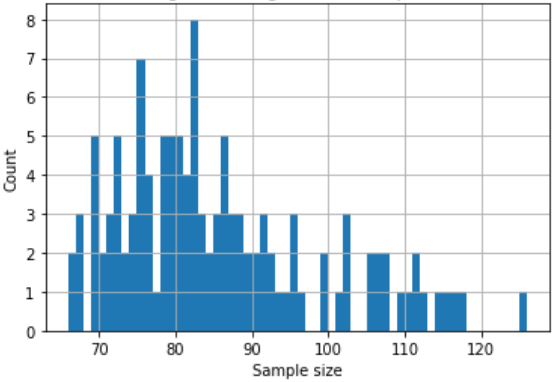
\includegraphics[width=8cm]{histo}
	\caption{Histogram of dog breeds' sample sizes}
	\label{fig:histo}
\end{figure}

Our baseline for classification is 11\% by naive guessing every outcome to be the most frequent class of Scottish Deerhound. For training purposes, the dataset is split into 80\% training and 20\% testing datasets. For neural networks, 10\% of training data is further reserved for validation data.

\begin{figure}[H]
	\centering
	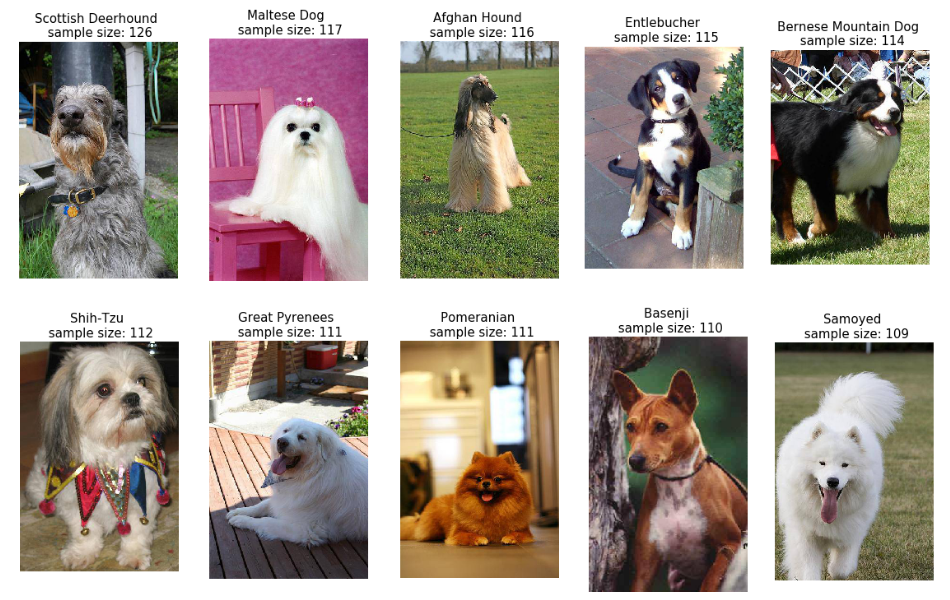
\includegraphics[width=11cm]{top10}
	\caption{Ten most frequent dog breeds in the dataset}
	\label{fig:top10}
\end{figure}

\section{Preprocessing}
\label{sec:prep}

In order to put the images into standardized dimensions, we use the OpenCV computer vision library and its included resize()-method. The corresponding relevant parameters are:

\begin{itemize}
	\item \textbf{src} - input image
	\item \textbf{dsize} - output image size
	\item \textbf{interpolation} - interpolation method
\end{itemize}

We resize all images (training and test data) to an output size of 150x150. Interpolation refers to the resampling method used to resize the images. Out of the given algorithms (nearest-neighbor interpolation, bilinear interpolation, resampling using pixel area relation, bicubic interpolation, Lanczos interpolation) we use the default bilinear interpolation.

\begin{figure}[h]
	\centering
	\begin{subfigure}[b]{5cm}
		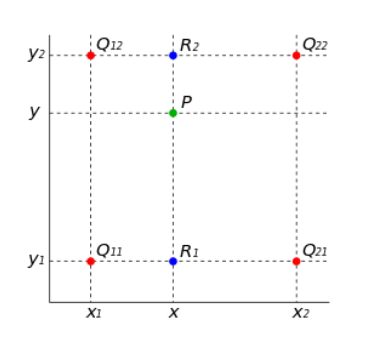
\includegraphics[width=5.5cm]{bilinear_up}
		\label{fig:up}
	\end{subfigure}
	\qquad
	\begin{subfigure}[b]{5cm}
		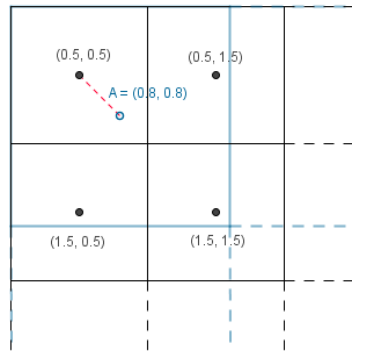
\includegraphics[width=5cm]{bilinear_down}
		\label{fig:down}
	\end{subfigure}
	\caption{Upsampling \cite{wiki:interpolation} and Downsampling \cite{sampling}}
	\label{fig:samp}
\end{figure}

Simply put, bilinear interpolation computes a new pixel value using the distance-weighted average of pixel values in the closest 2x2 neighborhood of known pixels. Given four points $Q_{1,1}, Q_{2,1}, Q_{1,2}, Q_{2,2}$ - as shown in Figure \ref{fig:samp} on the left - we want to interpolate $P$. We first get $R_1$ as the distance-weighted average of $Q_{1,1}$ and $Q_{2,1}$ and $R_2$ as the distance-weighted average of $Q_{1,2}$ and $Q_{2,2}$ and finally get $P$ as the distance-weighted average of $R_1$ and $R_2$. Scaling down works in the same way as upscaling (see Fig. \ref{fig:samp} on the right). The choice of interpolation method does not significantly affect accuracy scores of classification. 

Since all the images are of different sizes and aspect ratios, resizing to squared images of 150x150 causes distortion to various degrees. Regarding images of dogs, there are no geometric constraints and the defining characteristics seem to be the RGB values of the pixels rather than shapes. We therefore assume that this distortion does not have a significant effect on our success measures.

We will henceforth use these resized images, however each of the following methods applies further preprocessing steps.


\section{Data Mining}
\label{sec:class}

We first extracted features using Principal Component Analysis (PCA) in order to reduce dimensions for experimentation with different standard machine learning techniques. Variants of Neural Networks are then introduced with convolutional and pooling layers. Our discussion focuses on performance and loss metrics in addition to computational cost.

\subsection{Classic Classification Techniques}

\subsubsection*{Feature Extraction: PCA}
Colour images can be represented as 3D arrays consisting of 3 matrices that correspond to each of 3 colours in the RGB scheme. As images are highly dimensional data, it is advisable to compress them, reducing their sizes and at the same time retaining most of their qualities.
PCA is a technique which allows to transform a number of correlated variables into a smaller number of uncorrelated variables called principal components \cite{pca}. Each principal component is a linear combination of all original variables. The basis for the method is eigenvalues and eigenvectors of the covariance matrix calculated for the original data. Each eigenvalue corresponds to one principal component and is equal to its variation. The first principal component is created in a way to ensure that it contains as much of the variance of the original data as possible. Variance of each successive principal component is smaller than that of the preceding one. We applied principal component analysis on each colour value matrix. Values for columns of the images serve as variables for PCA.
In the case of our dataset, we flattened the images into one dimension and retained 50 principal components, which explain 73\% of total variance, where the first three components explain the 19.2\% 9.3\% and 6.2\%, respectively.

\subsubsection*{Standard Classifiers}
We started with some classic classification methods which were introduced in the lecture, namely KNN, Decision Trees and SVC. After implementing the basic model, we applied parameter tuning in form of an exhaustive grid search with cross validation on the possible parameters. 

\begin{table}[h]
	\centering
	\begin{tabular}{@{}ccc@{}}
		\toprule
		\textbf{Forecasting model}                                        & \textbf{Parameter name} & \textbf{Parameter value} \\ \midrule
		\multirow{2}{*}{\textbf{SVC}}                                     & kernel                  & 'linear'                 \\
		& C                       & 0.000125                 \\ \midrule
		\textbf{KNN}                                                      & n\_neighbors            & 29                       \\ \midrule
		\textbf{\begin{tabular}[c]{@{}c@{}}Decision\\ Trees\end{tabular}} & max\_depth              & 5                        \\ \bottomrule
	\end{tabular}
	\caption{Parameters of different classifiers}
	\label{tab:param}
\end{table}

Table \ref{tab:param} shows the optimal parameter setting derived from the grid search. We found out that most of the parameters for SVC, as well as for the decision trees remained equal to the default setting. 

\begin{figure}[h]
	\vspace{-10pt}
	\centering
	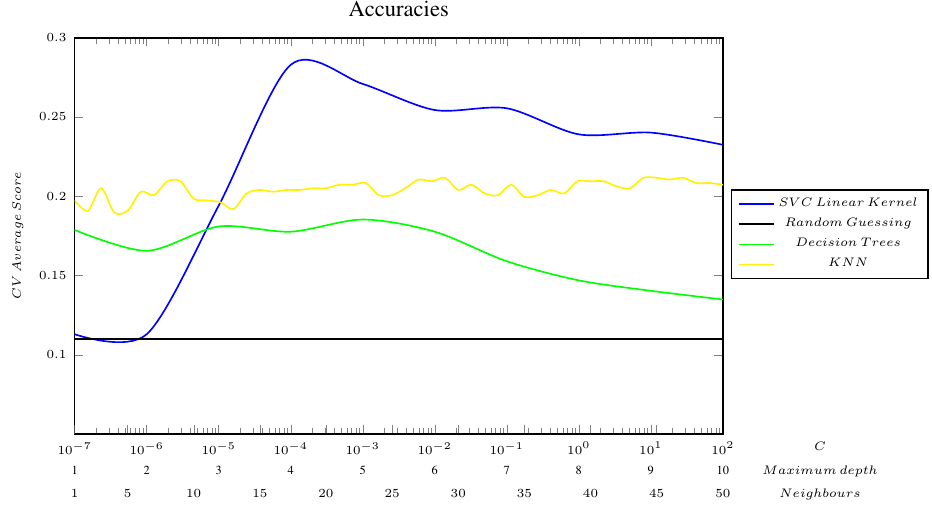
\includegraphics[width=12cm]{acc}
	\caption{Accuracy development}
	\label{fig:acc}
\end{figure}

Figure \ref{fig:acc} shows the accuracy development of the different classifiers when adapting the relevant parameters. One can clearly see that all methods show an improvement in comparison to the naive guessing baseline of 11\%. 

Table \ref{tab:acc} shows the accuracy score and the categorical cross entropy  using the best parameter settings for each model.
The highest accuracy within the basic classification models was achieved with the SVC, followed by KNN and Decision Trees. SVC generalizes well as they maximize the margin between hyperplanes. KNN instead is a so-called lazy learner, which means that it does not build an explicit model and simply uses the training data itself for classification, which makes it difficult to generate accurate forecasts for high-dimensional data. The poor performance of the Decision Trees can be explained by the fact that they can only represent decision boundaries that are parallel to the axes, which might be difficult for high dimensional data.
Furthermore, Table \ref{tab:acc} shows the prediction and computational changes when applying PCA. It shows that the main improvement of the PCA in our case is computational, decreasing e. g. the fitting time of SVC from about 15 minutes to less than a minute, while the prediction accuracy remains roughly the same.
Additionally, it must be mentioned that we had a very small training data set, which surely had a negative impact on the prediction accuracy of the different classifiers. 

\begin{table}[]
	\vspace{-10pt}
	\centering
	\begin{tabular}{@{}cc|ccc@{}}
		\toprule
		&                                                                       & \textbf{SVC}                    & \textbf{KNN}                    & \textbf{\begin{tabular}[c]{@{}c@{}}Decision\\ Trees\end{tabular}} \\ \midrule
		\multirow{3}{*}{\textbf{with PCA}}    & \textbf{\begin{tabular}[c]{@{}c@{}}Categorical\\ Cross\\ Entropy\end{tabular}} & 1.9969                 & 4.8037                 & 2.8704                                                   \\ \cmidrule(l){2-5}
		& \textbf{Accuracy Score}                                                        & 0.2764                 & 0.1712                 & 0.2022                                                   \\ \cmidrule(l){2-5}
		& \multicolumn{1}{l|}{\textbf{Fitting Time (sec)}}                               & \multicolumn{1}{l}{0.8745} & \multicolumn{1}{l}{0.0041} & \multicolumn{1}{l}{0.0396}                                   \\ \midrule
		\multirow{3}{*}{\textbf{without PCA}} & \textbf{\begin{tabular}[c]{@{}c@{}}Categorical\\ Cross\\ Entropy\end{tabular}} & 1.9948                 & 6.9274                 & 4.1486                                                   \\ \cmidrule(l){2-5}
		& \textbf{Accucary Score}                                                        & 0.2751                 & 0.1838                 & 0.1891                                                   \\ \cmidrule(l){2-5}
		& \multicolumn{1}{l|}{\textbf{Fitting Time (sec)}}                               & \multicolumn{1}{l}{873.5343} & \multicolumn{1}{l}{5.2452} & \multicolumn{1}{l}{41.6183}                                   \\ \bottomrule
	\end{tabular}
	\caption{Accuracies for standard classifiers}
	\label{tab:acc}
\end{table}

\subsection{Convolutional Neural Networks}
This section introduces the fundamental concepts of Convolutional Neural Networks - henceforth CNNs - that are widely applied in the field of image recognition, followed by graphical presentations of our network architecture and the learning process. 

\subsubsection*{Convolution}
In traditional neural networks, each layer employs matrix multiplication on weights, biases and inputs to proceed to the next layer with a given activation function. CNNs replace at least one of those layers with an operation called convolution, where two functions f and g are transformed into a third function f*g which can be viewed as a modified version of either f or g. In the context of image recognition, f is a multidimensional array of image input that is typically width, height and color channels, while g is called the kernel which specifies the size of local regions and weights associated with the corresponding pixel. The following shows the first operation of convolution on input of 4*3 array and 2*2 kernel that is a simple weighted average, which keeps iterating over each 2*2 region in the input space leading to the output of size 3*2. There are H different output layers where H is the number of variations of the kernel which is actively learned \cite{G16}. Intuitively, convolution can be viewed as a local feature extractor, and while early convolutional layers extract simple features such as edges and shadows, more ambiguous features such as nose shape are picked up in later layers.

\subsubsection*{Pooling}
Convolutional layers are typically followed by pooling layers which downsize the feature resolutions. For a given size of pooling window, pooling takes either the average or the maximum value of the region. Applying $2\times2$ pooling on the input of size $4\times4$ divides the input into four non-overlapping matrices, where integers represent the magnitude of a given colour channel (Figure 2). Pooling is beneficial as they reduce memory usage and lower sensitivity to overfitting.

\begin{figure}[h]
	\centering
	\begin{subfigure}[b]{6cm}
		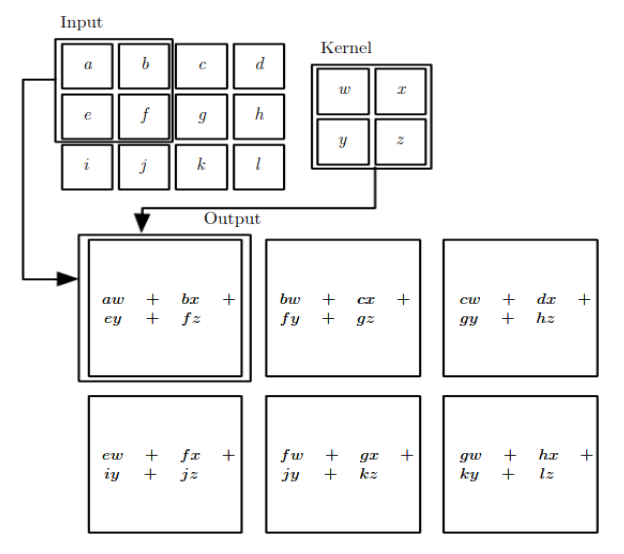
\includegraphics[width=6cm]{conv}
	\end{subfigure}
	~
	\begin{subfigure}[b]{6cm}
		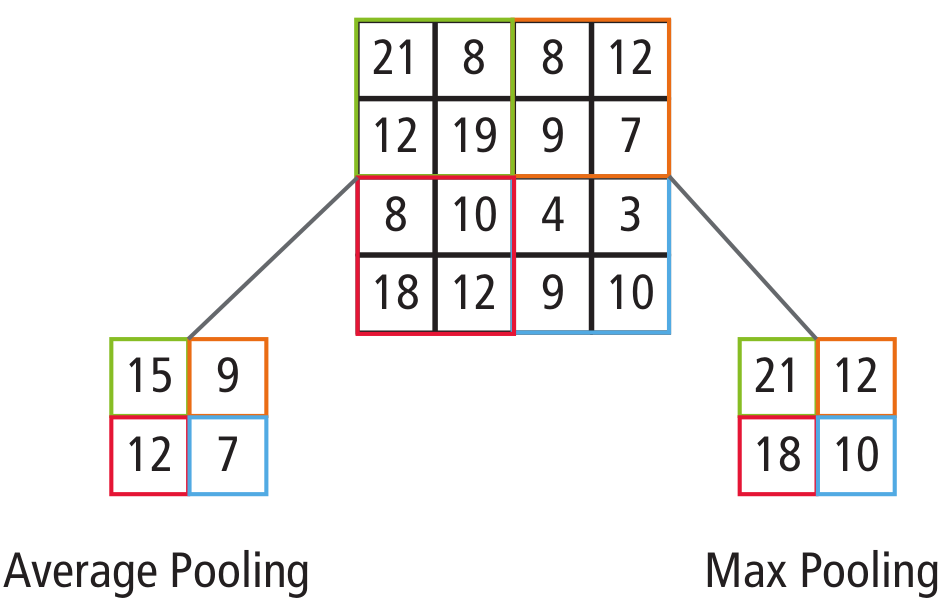
\includegraphics[width=6cm]{pool}
	\end{subfigure}
	\caption{Convolution \cite{G16} and Pooling \cite{H15}}
	\label{fig:convpool}
\end{figure}

\subsubsection*{Architecture}

Our CNN implementation basically follows the one proposed by Le Cun et al. \cite{L90} for digits recognition, with three convolutional layers followed by $2\times2$ max pooling. Exceptions include the use of ReLu as activation function $(f(x) = \max \{0,x\})$ and the addition of Dropout layer which selects random portion of the data for training at each epoch to avoid overfitting, which is 50\%. The network is graphically represented as follows, where activation function for convolutional layers are ReLU except for the last fully connected layer where softmax is used to output probabilities.

\begin{figure}[h]
	\centering
	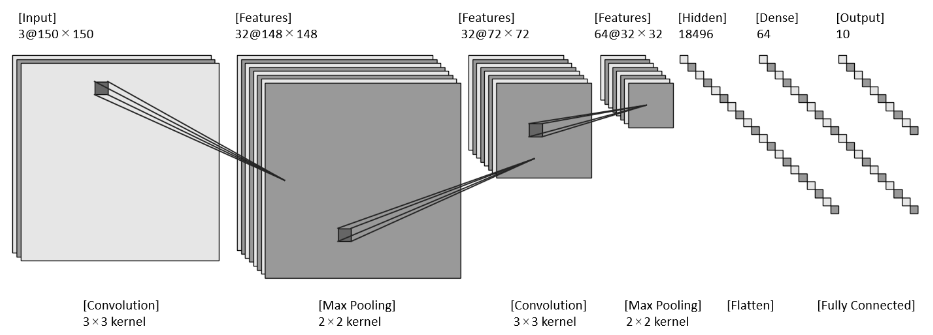
\includegraphics[width=10cm]{arch}
	\caption{CNN architecture}
	\label{fig:arch}
\end{figure}

Additionally, as part of preprocessing, images are randomly rotated by up to 20 degrees, horizontally flipped, and zoomed by up to 20\%. Shear transformation is also performed, which is a linear mapping of images that displaces pixels horizontally by up to 20\%. These processes are applied only to training data to improve generality of the model, and new image is generated at each batch. Sample images generated by this process are shown below.

\begin{figure}[h]
	\centering
	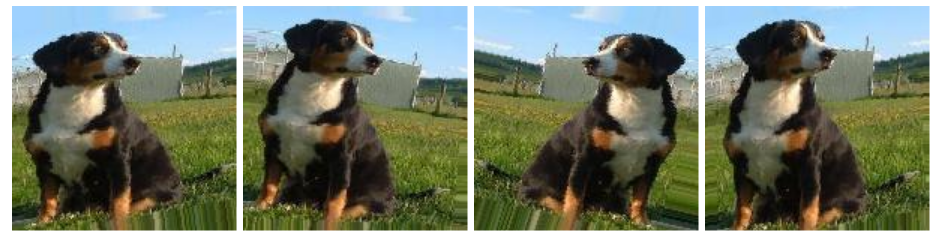
\includegraphics[width=12cm]{trans}
	\caption{rotated, flipped, and zoomed}
	\label{fig:trans}
\end{figure}

Dataset is split into training, validation and testing datasets where test size is 20\% of the whole dataset and validation is 10\% of the training dataset, where the absolute sizes of each are 820, 92 and 229 respectively. Training is run for 50 epochs with adam as optimizer as suggested by Kingma and Ba \cite{KB14} and categorical cross entropy as objective function to minimize. Image size is 150x150 as per the case of PCA and standard classifiers. The learning process is visualised as follows in Figure \ref{fig:learn}. While training error and accuracy are converging to 0 and 1, validation error was minimum at 1.46 and accuracy was highest at 0.58. The model starts to overfit after 15-20 epochs, where validation accuracy does not improve more than roughly 0.5.  
Note, however, that the small size of validation data at 92 belonging to 10 classes might not be sufficiently large enough to use as a reference for learning. Final evaluation with the testing dataset yields categorical cross entropy loss of 1.79 with accuracy of 0.45, which is a significant improvement from 1.99 and 0.28 with PCA and SVC. Although CNNs take more time to train than traditional machine learning techniques with approximately 70 minutes with CPU, it is evident that the performance justifies the computational cost. 

\begin{figure}[h]
	\centering
	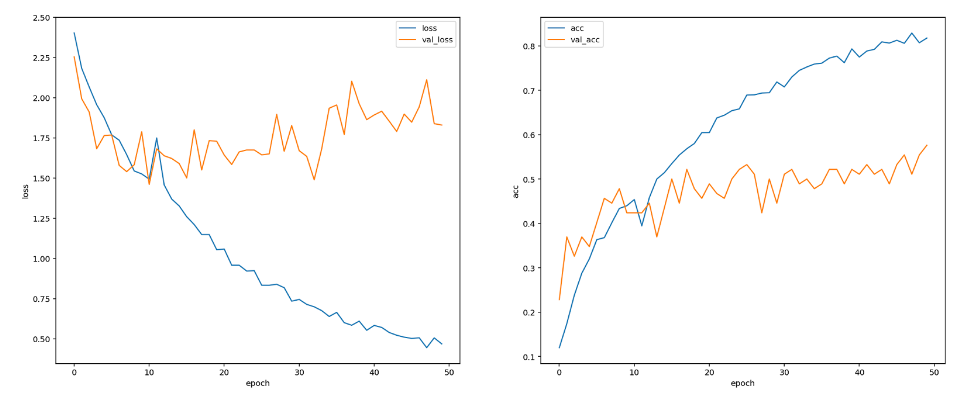
\includegraphics[width=10cm]{learning}
	\caption{Learning process of CNN}
	\label{fig:learn}
\end{figure}

\subsection{Transfer Learning and InceptionV3}

This section introduces the concept of transfer learning, and show that it is highly applicable to our task yielding high accuracy. As explained earlier, early convolutional layers detect local features such as shadows and edges, and they are most likely to be useful for other image classification tasks. Transfer learning allows one to store knowledge gained in solving problems in one domain and apply to relevant tasks in other areas \cite{R17}. In our application, we employ a pre-computed network called InceptionV3 as a feature extractor for our dog breed dataset, and classify the features into 10 classes by implementing the last fully-connected layer with softmax as activation function. InceptionV3 \cite{inc15} is a variant of deep convolutional neural networks trained on ImageNet dataset containing 1.2 million images with 1000 classes. Figure \ref{fig:incep} shows schematic visualisation of the InceptionV3 architecture, which iconically includes inception modules where layers go through several convolutional filters in parallel and are concatenated into one layer.

\begin{figure}[h]
	\centering
	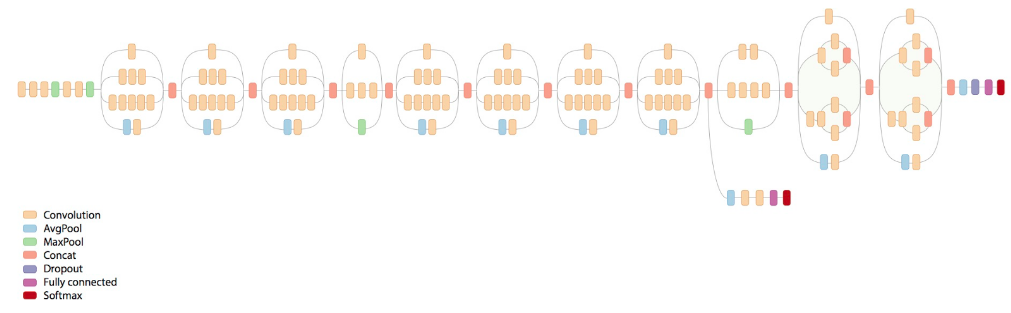
\includegraphics[width=12cm]{inception}
	\caption{InceptionV3 architecture}
	\label{fig:incep}
\end{figure}

\subsubsection*{Result and Discussion}
Figure \ref{fig:learn2} shows the learning process of the last layer with 50 epochs where categorical cross entropy is minimised and adam is used as optimiser as per the previous CNN implementation. Validation loss lowest at 0.73 and accuracy is highest at 0.86. Final evaluation with the testing dataset is loss of 0.78 and accuracy of 0.85, which is a significant improvement from our result with CNN. Transfer learning with a pre-computed network was computationally extremely efficient as feature extraction took roughly 5 minutes for the entire dataset and the final layer was trained less than a second for each epoch. Despite the lack of flexibility in terms of model improvement and its blackbox nature, transfer learning appears to be very powerful in recognizing objects and extracting features. Generality to other domain-specific images is however still uncertain, as it is possible that there are objects not contained or properly classified in the original ImageNet dataset.

\begin{figure}[h]
	\centering
	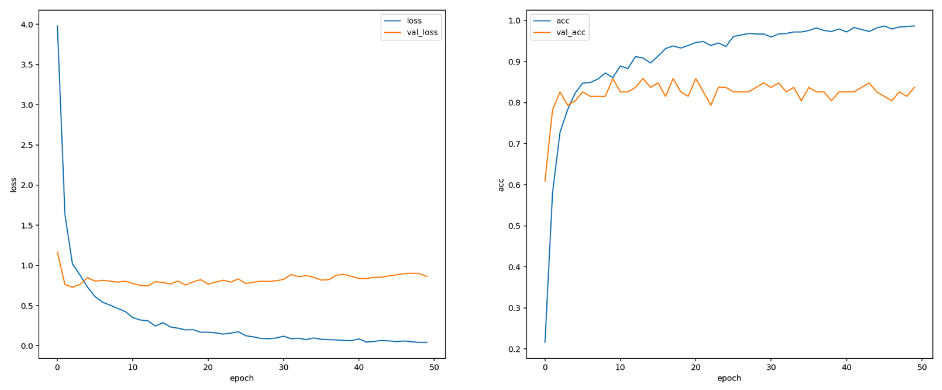
\includegraphics[width=10cm]{learning2}
	\caption{Learning process of last layer of InceptionV3}
	\label{fig:learn2}
\end{figure}

\section{Conclusion}
We demonstrated that PCA improves computational efficiency while retaining the predictive power with the highest of 27\% accuracy with SVC against the naive baseline of 11\%. Despite the longer training time of 70 minutes, our CNN implementation excels at image classification with accuracy score of 45\%, and transfer learning with Inception proves to be extremely powerful with 85\%.

\newpage

\bibliographystyle{plain}
\bibliography{references}

\end{document}
